\documentclass[aspectratio=169]{beamer}
\usepackage{fontspec}
\usepackage{hyperref}
\usepackage{ccicons}
\protrudechars=2 % or \pdfprotrudechars=2 and
\adjustspacing=2 %    \pdfadjustspacing=2 with luatex < v0.85
\usepackage{amsmath}
\usepackage{graphicx}
\usepackage[table]{xcolor} % Για χρωματισμούς στις γραμμές και τις στήλες
\usepackage{xcolor}
\usepackage{polyglossia}
\usepackage{csquotes}
\usepackage[symbol]{footmisc}
\setmainlanguage{greek}
\setotherlanguage{english}
\setmainfont[Numbers={OldStyle, Proportional},
Ligatures=TeX]{Linux Libertine O}
\newfontfamily\greekfont{Linux Libertine O}
\newfontfamily\englishfont{Linux Libertine O}
\newfontfamily\greekfontsf{Linux Libertine O}
\usetheme{Madrid}
\usecolortheme{beaver}
\title{Εισαγωγή στο λογισμικό της διαδικτυακής αναμετάδοσης}
\subtitle{\href{https://obsproject.com/}{OBS (Open Broadcaster Software)} και πλατφόρμες διαδικτυακής αναμετάδοσης} 
\author{Ερμής Δούλος (\textit{dit17046@uop.gr})}
\begin{document}
\section{intro}
\begin{frame}
  \titlepage
  \begin{center}
    % GitHub Link
    \href{https://github.com/doblador42}{\textbf{Github Profile:}}\\
    % QR Code
    
\includegraphics[width=0.13\textwidth]{images/qrcode.png}
  \end{center}
\end{frame}
\begin{frame}{Περιεχόμενα}
  \tableofcontents
\end{frame}

\section{Επισκόπηση}
\begin{frame}{Επισκόπηση}
  \begin{block}{Περιεχόμενα}
    \begin{itemize}
      \item Ανασκόπηση του λογισμικού μιας τηλεμετάδοσης
      \item Εισαγωγή στο \href{https://obsproject.com/}{OBS}
            \begin{itemize}
              \item Εγκατάσταση
              \item Ρύθμιση
              \item Χρήση
                    \begin{itemize}
                      \item Πηγές
                      \item Σκηνές
                      \item Επιλογές διάταξης
                    \end{itemize}
            \end{itemize}
      \item Πλατφόρμες αναμετάδοσης
            \begin{itemize}
              \item \href{https://www.youtube.com/}{YouTube}
              \item \href{https://zoom.us/}{Zoom}
              \item \href{https://www.webex.com/}{Webex}
              \item \href{https://www.microsoft.com/el-gr/microsoft-teams/group-chat-software}{Teams}
            \end{itemize}
      \item Παραδείγματα
    \end{itemize}
  \end{block}
\end{frame}
\subsection{διάγραμμα διάταξης αναμετάδοσης}
\begin{frame}{Διάγραμμα όλης της αναμετάδοσης}
  \begin{figure}
    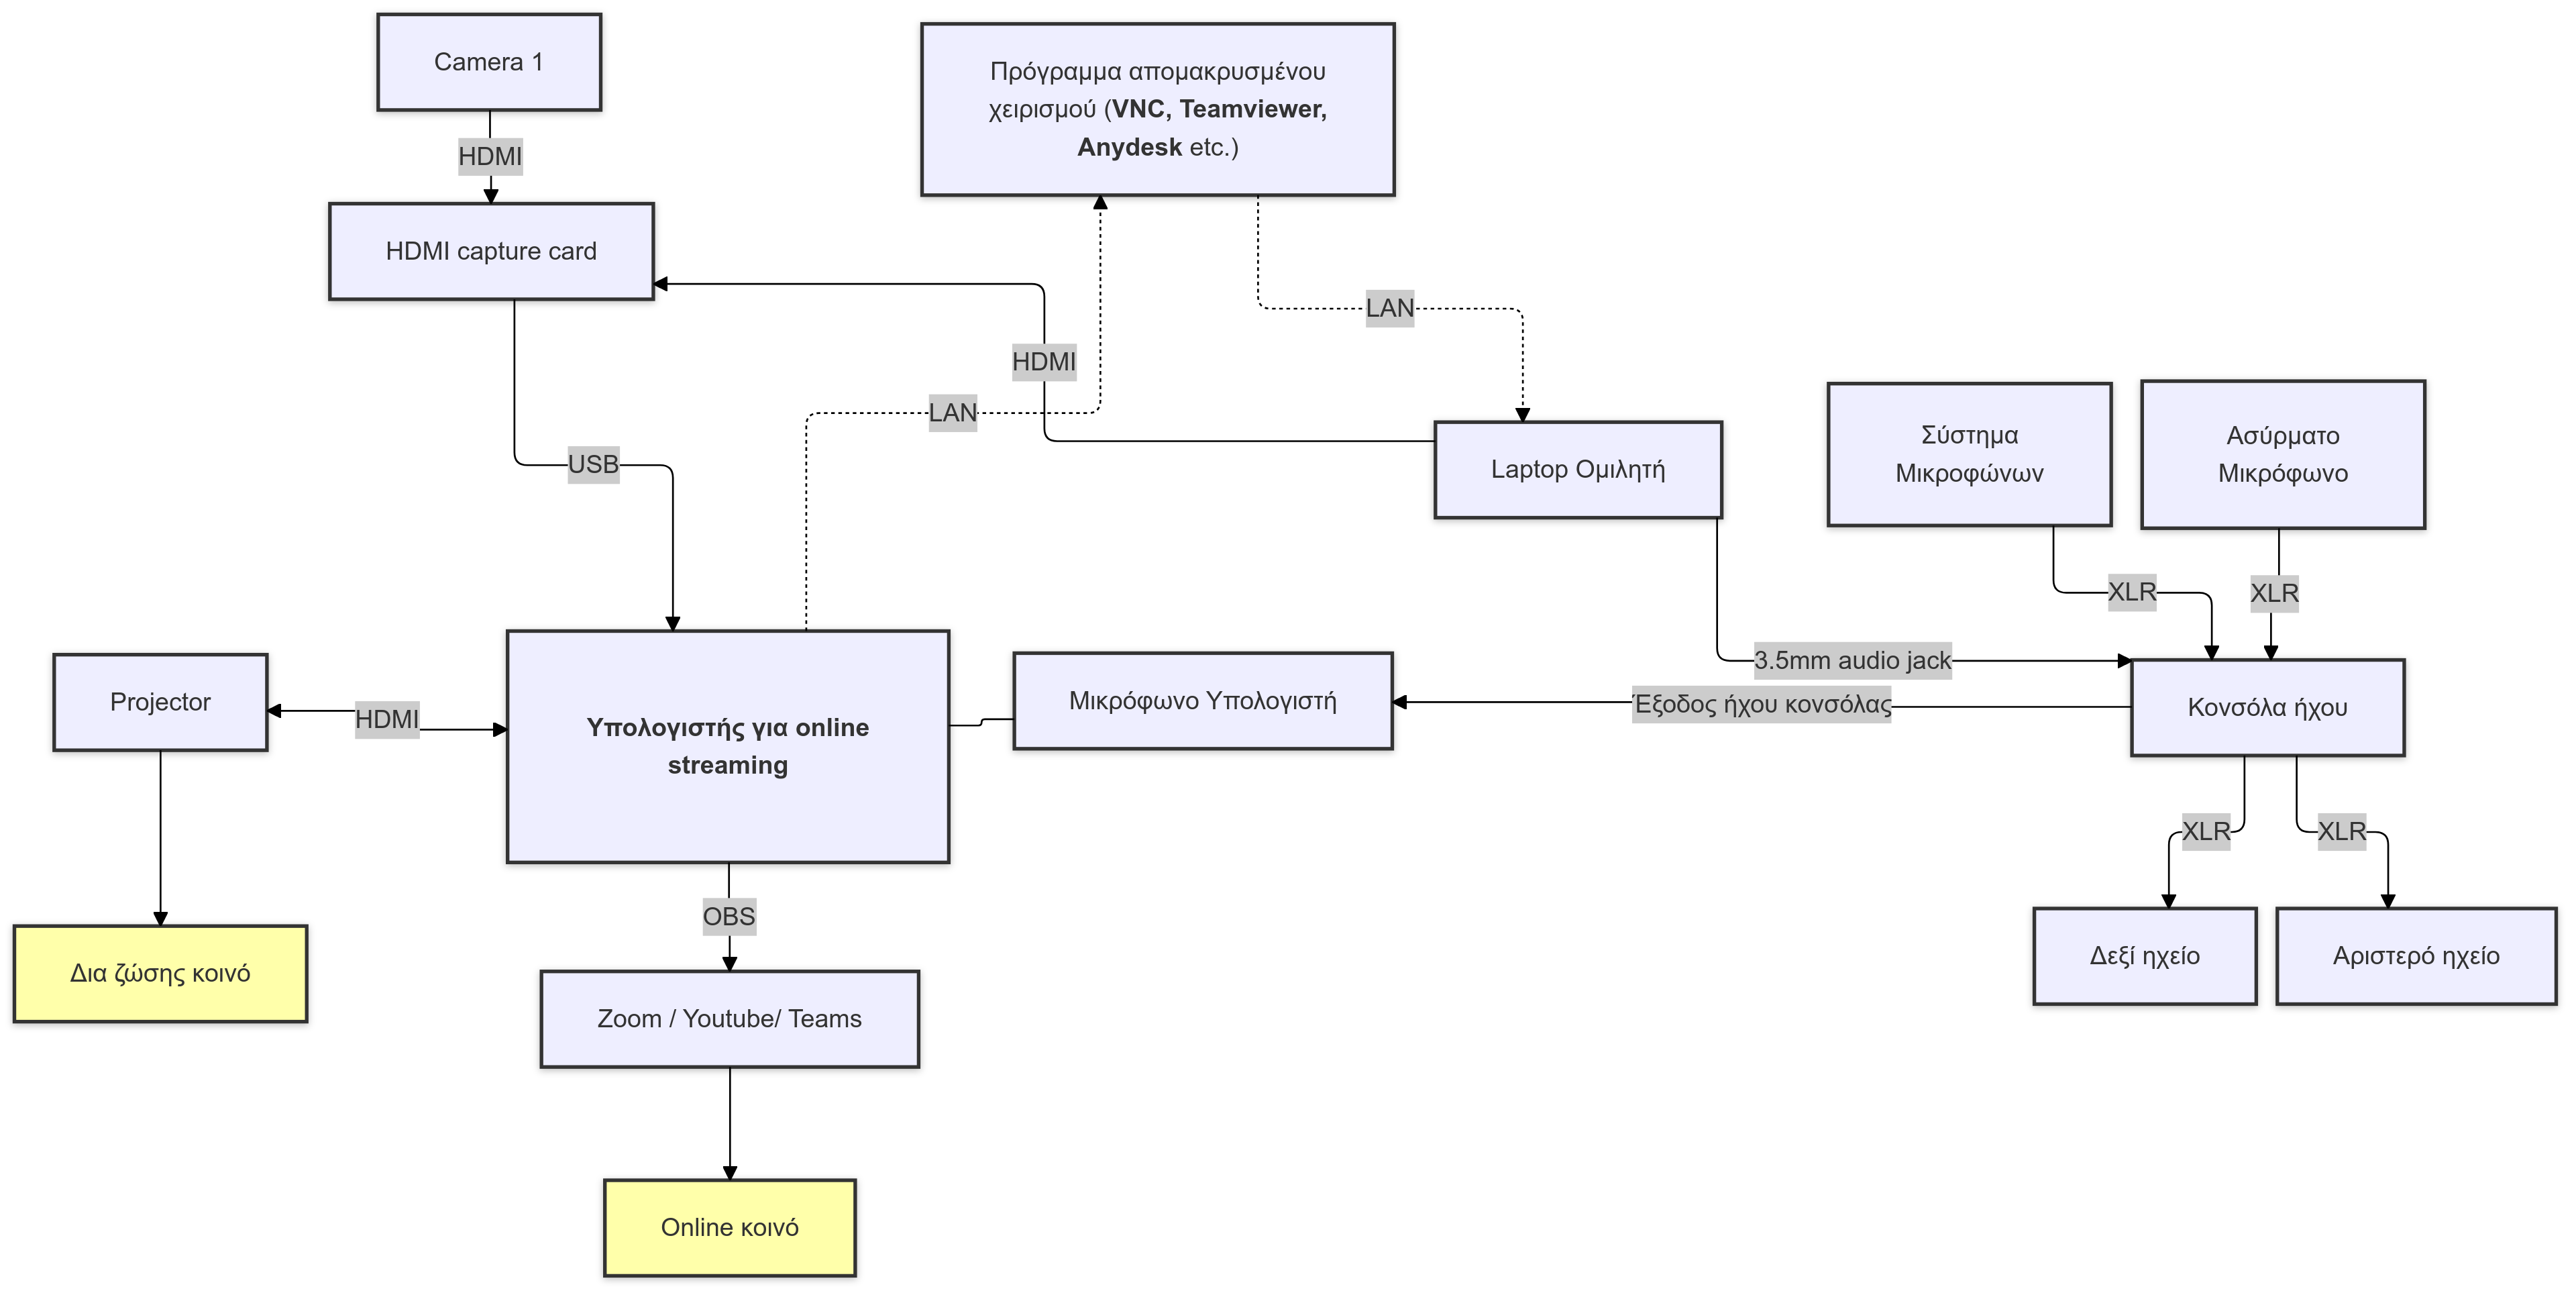
\includegraphics[width=0.8\textwidth]{images/diagram.png}
    \caption{Διάγραμμα όλης της αναμετάδοσης}
    \label{fig:diagram}
  \end{figure}
\end{frame}
\subsection{διάγραμμα του αντικειμένου μας για σήμερα}
\begin{frame}{Με τι θα ασχοληθούμε σε αυτό το session;}
  \begin{block}{Η διάταξη που θα μας απασχολήσει σήμερα:}
    \begin{figure}
      % full fledged figure with caption and label
      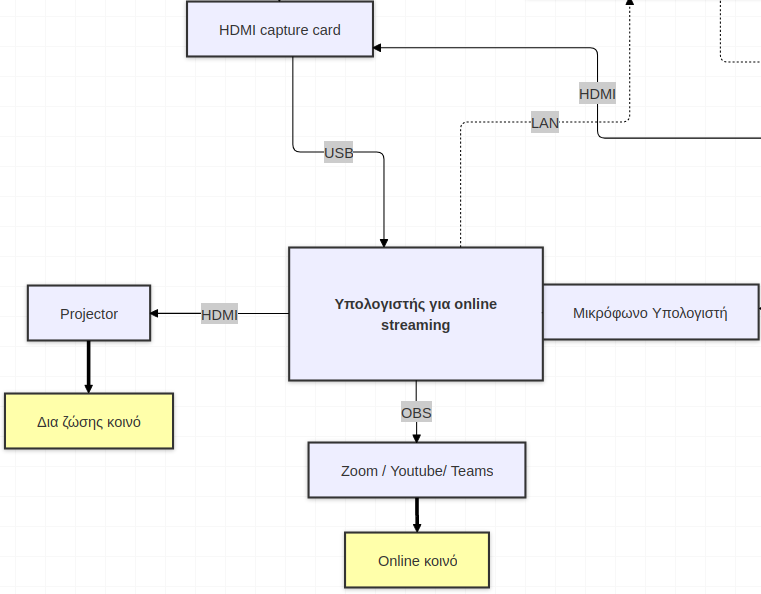
\includegraphics[width=0.42\textwidth]{images/laptop.png}
      \caption{Διάταξη που μας απασχολεί στο σημερινό session}
      \label{fig:laptop}
    \end{figure}
  \end{block}
\end{frame}
\section{Πρόγραμμα για live-streaming;}
\subsection{τι είναι αυτά που ζητάμε;}
\begin{frame}{Τι χρειαζόμαστε για μια διαδικτυακή αναμετάδοση;}
  \begin{block}{Πρόγραμμα αναμετάδοσης}
    \begin{itemize}
      \item Εύκολη χρήση\footnote{Χωρίς πολύπλοκες ρυθμίσεις και προσβάσιμο και σε μη ειδικούς}
      \item Ευελιξία\footnote{Δυνατότητα προσθήκης πολλαπλών πηγών και παραμετροποίησης της εμφάνισης τους}
      \item Επαγγελματική ποιότητα\footnote{Καλή ποιότητα εικόνας και ήχου χωρίς διαλείψεις και εκπλήξεις}
      \item Ελεύθερο λογισμικό\footnote{Διότι είναι δωρεάν και ανοιχτού κώδικα}
    \end{itemize}
  \end{block}
\end{frame}
\subsection{Δημοφιλή προγράμματα αναμετάδοσης}
\begin{frame}{Λογισμικό αναμετάδοσης}
    \begin{columns}
      \begin{column}{0.4\textwidth}
        \begin{exampleblock}{Προτεινόμενο λογισμικό}
        \begin{itemize}
          \item \textbf{\href{https://obsproject.com/}{OBS (Open Broadcaster Software)}}
          \item \href{https://www.xsplit.com/}{XSplit}
          \item \href{https://streamlabs.com/}{Streamlabs OBS}
          \item \href{https://www.telestream.net/wirecast/}{Wirecast}
          \item \href{https://www.vmix.com/}{vMix}
        \end{itemize}
      \end{exampleblock}
      \end{column}
      \begin{column}{0.6\textwidth}
        \begin{center}
          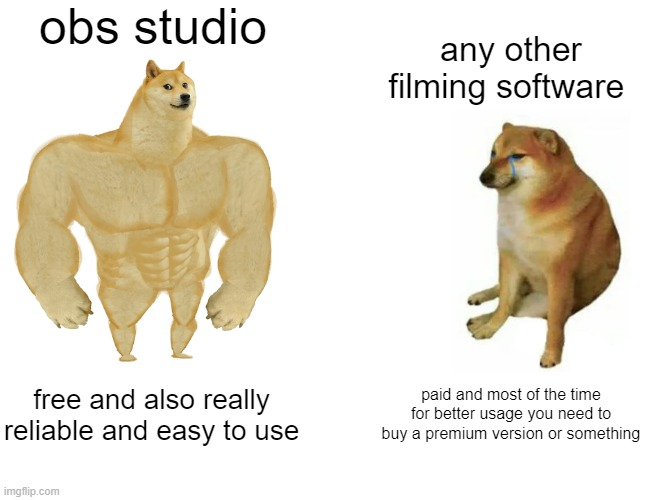
\includegraphics[width=0.9\textwidth]{images/meme.jpg}
        \end{center}
      \end{column}
    \end{columns}
\end{frame}
\section{Το OBS}
\subsection{Εισαγωγικές πληροφορίες;}
\begin{frame}{Τι είναι το OBS και γιατί το χρειαζόμαστε;}
  \begin{block}{Ορισμός}
    Το \textbf{\href{https://obsproject.com/}{Open Broadcaster Software}} είναι ένα λογισμικό ανοιχτού κώδικα που χρησιμοποιείται
    για τοπική καταγραφή και αναμετάδοση περιεχομένου σε πλατφόρμες όπως το \href{https://www.youtube.com/}{YouTube},
    το \href{https://www.twitch.tv/}{Twitch}, το \href{https://www.facebook.com/}{Facebook} και το \href{https://twitter.com/}{Twitter}.
  \end{block}
  \begin{block}{Χρησιμότητά του για εμάς}
    Για εμάς το \textbf{OBS} είναι ένα εργαλείο που μας επιτρέπει να μοιραστούμε \textbf{διαδικτυακά} το τι γίνεται μέσα στο \textbf{αμφιθέατρο}
    της σχολής μας, χρησιμοποιώντας τις \textbf{κάμερες}, τα \textbf{μικρόφωνα} όλης της αίθουσας και τις \textbf{παρουσιάσεις} που γίνονται σε αυτό.
    Κύρια πλεονεκτήματά του είναι πως είναι \textbf{δωρεάν} και \textbf{ανοιχτού κώδικα}, καθώς επίσης πως είναι \textbf{δοκιμασμένο} και \textbf{αξιόπιστο}.
  \end{block}
\end{frame}
\subsection{Εγκατάσταση}
% Installation Slide
\begin{frame}{Εγκατάσταση του OBS}
  \begin{columns}
    \begin{column}{0.8\textwidth}
      \begin{block}{Ελάχιστες Απαιτήσεις Συστήματος}
        \begin{itemize}
          \item \textbf{Λειτουργικό Σύστημα:} Windows 10 ή νεότερο, macOS 10.13 ή νεότερο, Linux
          \item \textbf{Επεξεργαστής:} Intel Core i5 6ης γενιάς ή νεότερος ή αντίστοιχος AMD
          \item \textbf{Μνήμη RAM:} 8GB ή περισσότερο
          \item \textbf{Κάρτα Γραφικών:} DirectX 11.1 / OpenGL 3.3 capable ή νεότερο\footnote{Μερικές φορές όπως στη δική μας περίπτωση, η ενσωματωμένη κάρτα γραφικών είναι αρκετή.}
        \end{itemize}
      \end{block}
      \begin{block}{Εγκατάσταση}
        Κατεβάστε το \textbf{OBS} από την επίσημη ιστοσελίδα: \href{https://obsproject.com/}{obsproject.com}
      \end{block}
    \end{column}
    \begin{column}{0.2\textwidth}
      \begin{center}
        
\includegraphics[width=0.95\textwidth]{images/obs2.png}
      \end{center}
    \end{column}
  \end{columns}
\end{frame}
\subsection{Διεπαφή και ρύθμιση}
\begin{frame}[allowframebreaks]{Η διεπαφή του OBS}
  \begin{block}{Αρχική οθόνη}
    \begin{figure}
      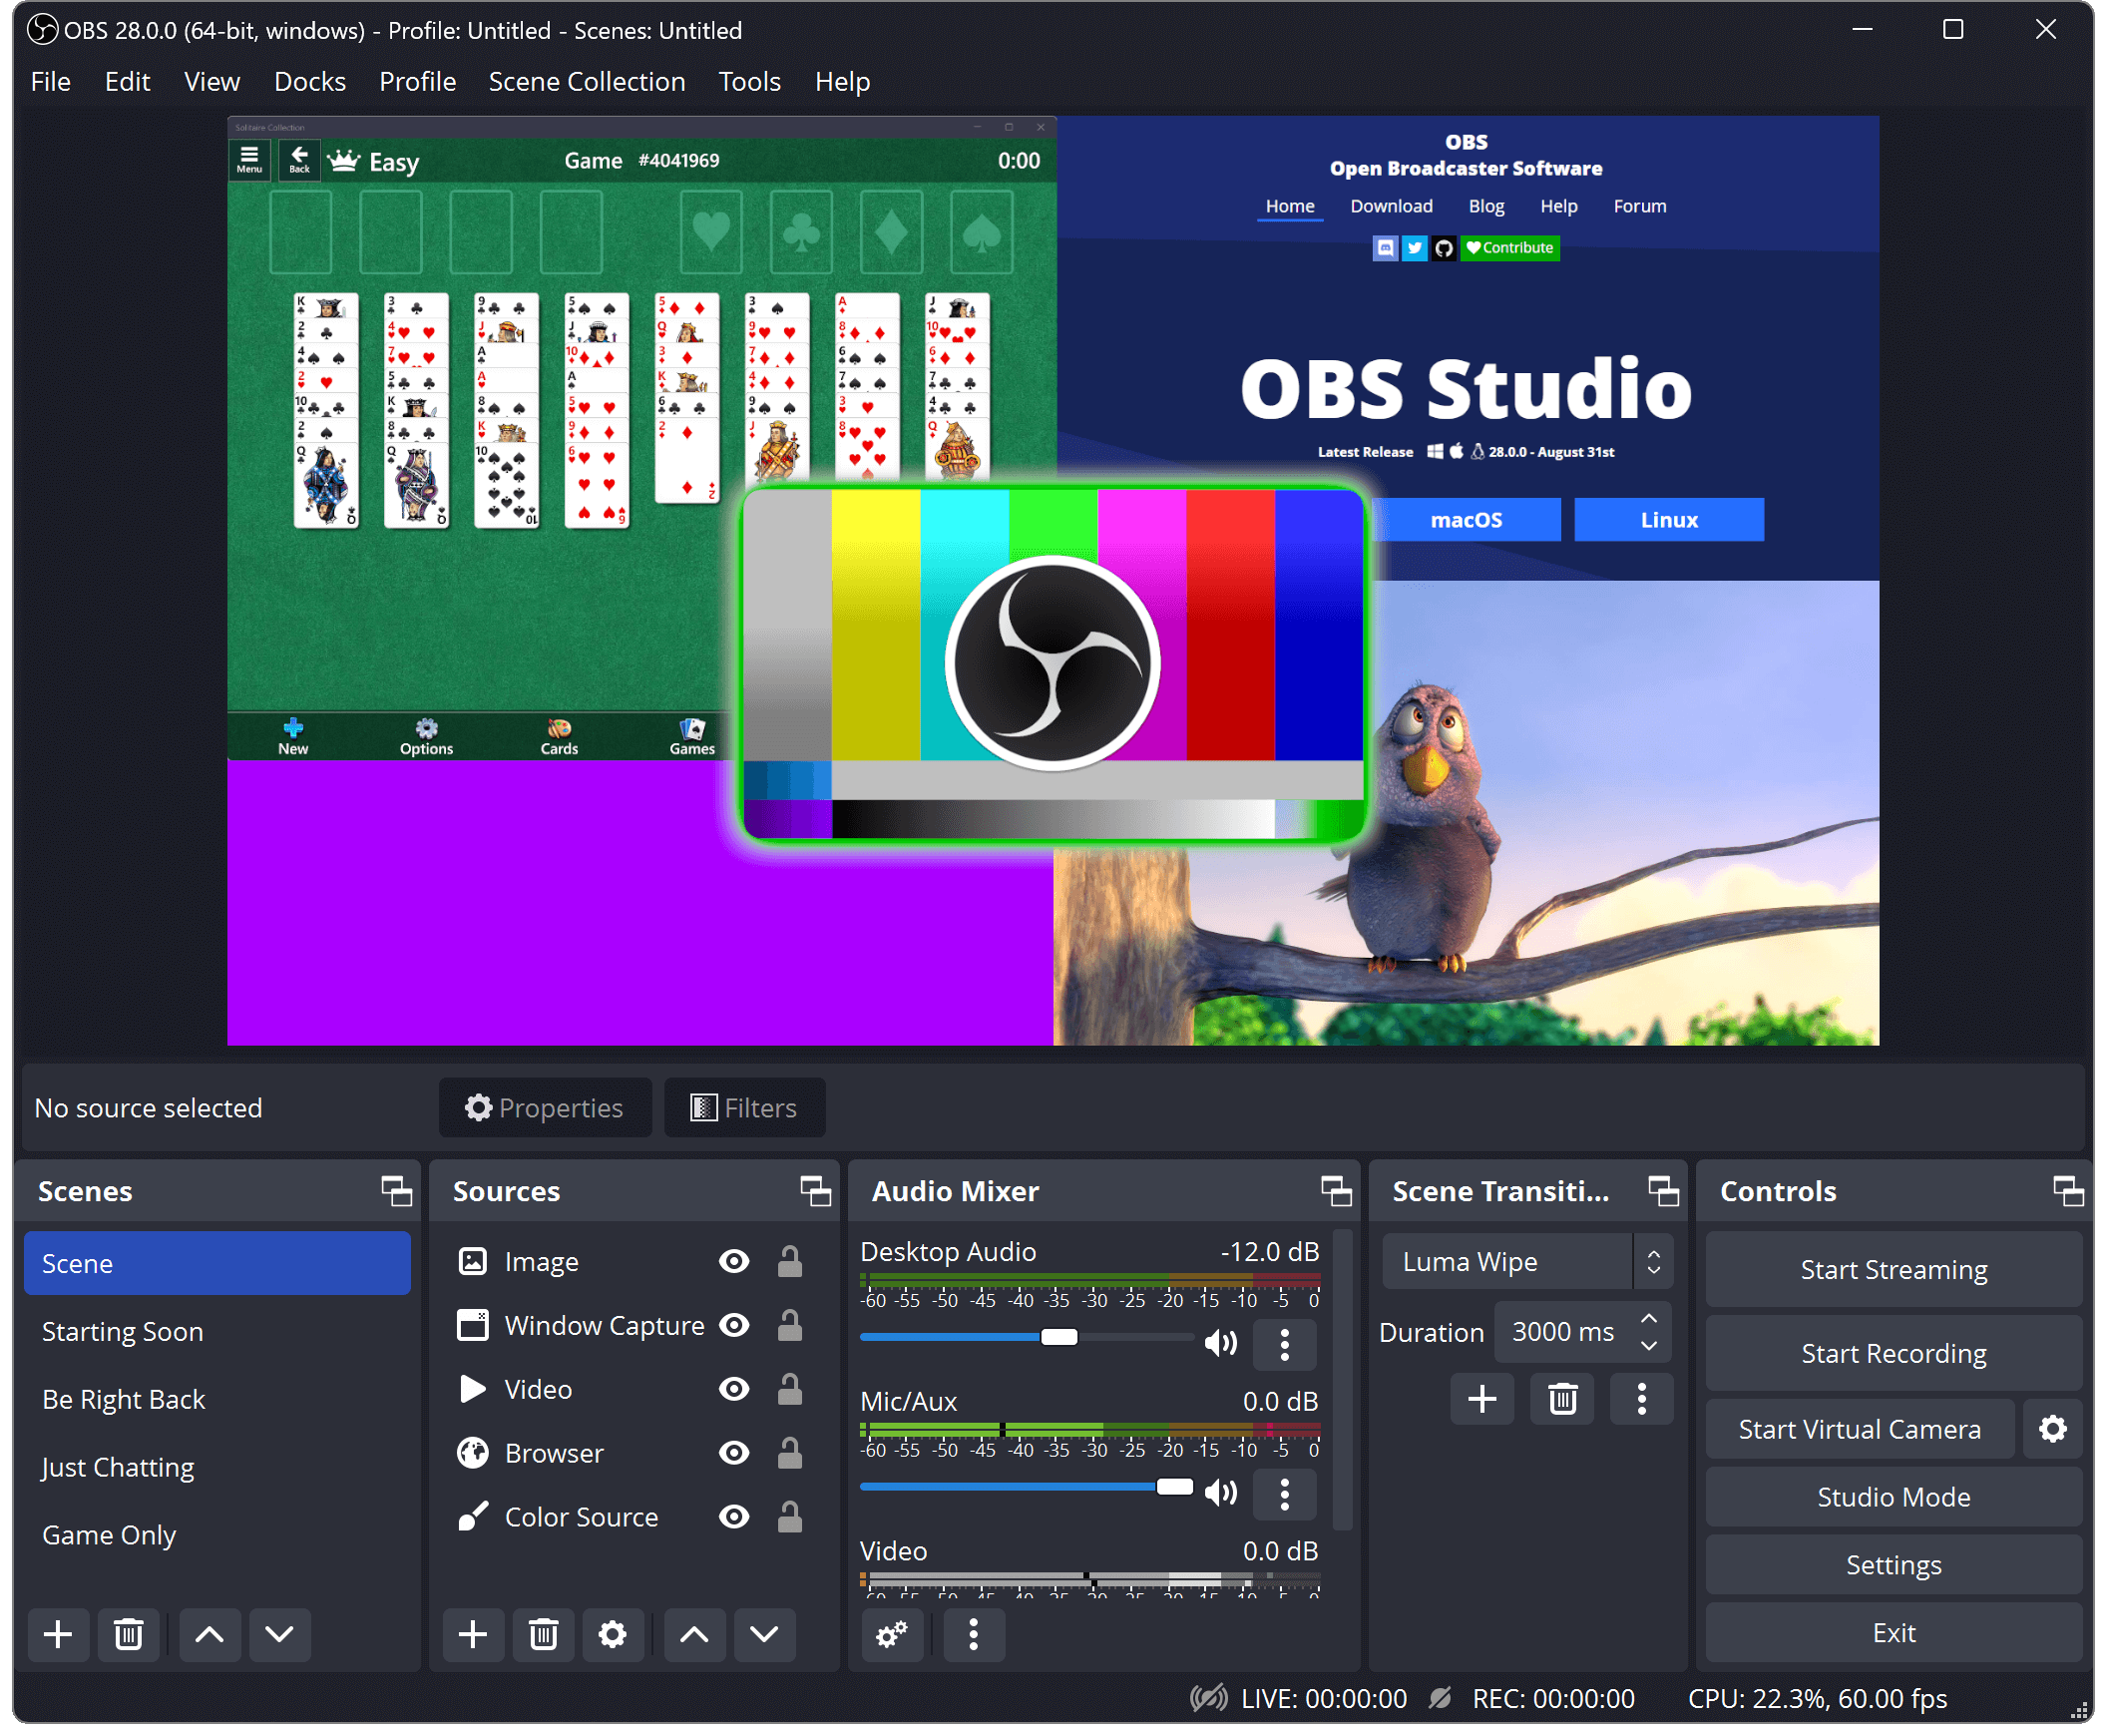
\includegraphics[width=0.38\textwidth]{images/screenshot_obs.png}
      \caption{Η κύρια οθόνη του OBS Studio}
      \label{fig:obs_interface}
    \end{figure}
  \end{block}
  \begin{block}{Επιλογές στη βασική οθόνη}
    \begin{figure}
      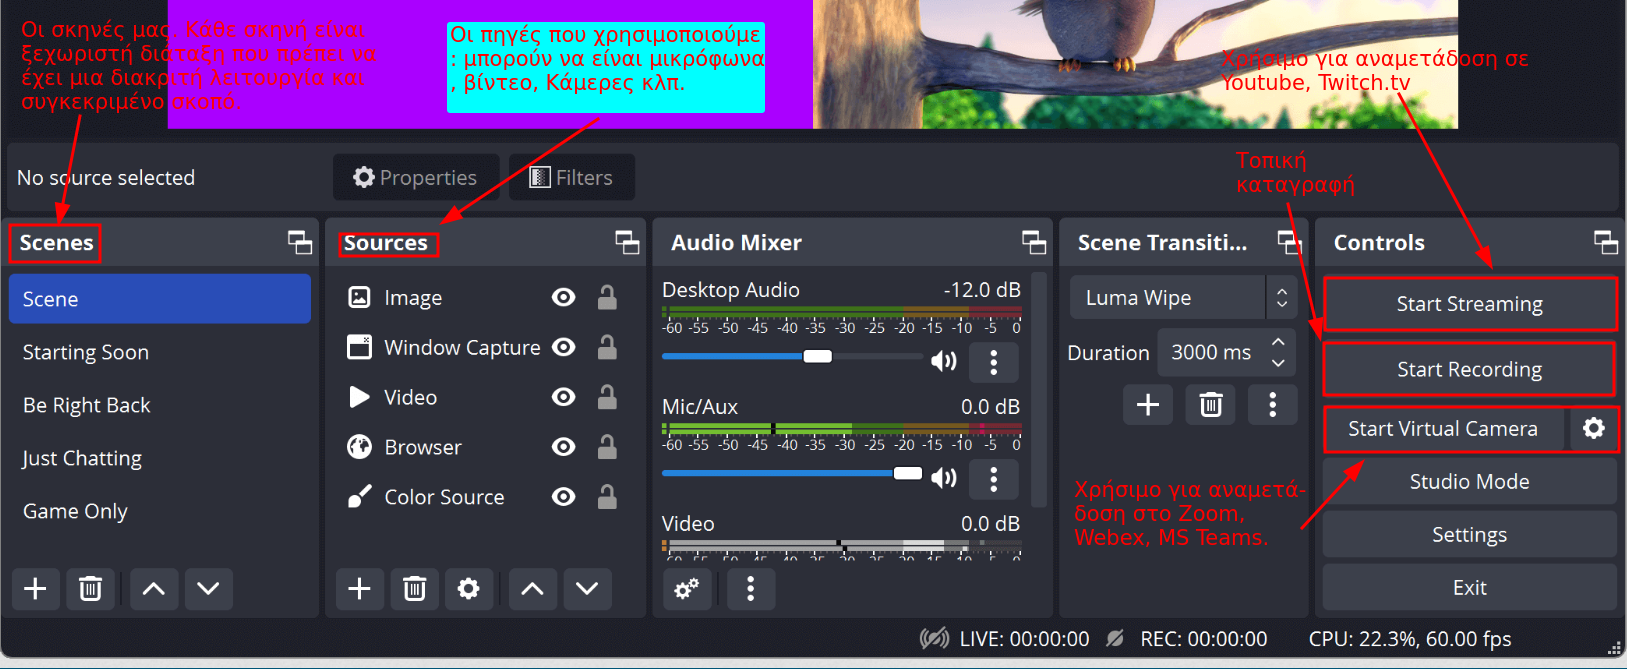
\includegraphics[width=0.8\textwidth]{images/obs_tools.png}
      \caption{Η οθόνη ρύθμισης του OBS Studio}
      \label{fig:obs_interface2}
    \end{figure}
  \end{block}
\end{frame}
\section{Συνάντηση δια-ζώσης}
\begin{frame}[allowframebreaks]{Εξάσκηση στο OBS}
  \begin{alertblock}{Πότε και πού}
    \begin{itemize}
      \item \textbf{Ημερομηνία:} Τρίτη, 3 Δεκεμβρίου 2024
      \item \textbf{Ώρα:} 3:00 μ.μ.
      \item \textbf{Τοποθεσία:}
        \begin{itemize}
          \item Εργαστήριο CNA LAB
          \item Πάνω όροφος
          \item Κάτω κτήριο Σχολής Επιστημών και Τεχνολογίας
        \end{itemize}
    \end{itemize}
  \end{alertblock}
\end{frame}

\begin{frame}{Ευχαριστώ για την προσοχή σας!}
  \begin{columns}
    \begin{column}{0.4\textwidth}
      \begin{center}
        \Huge{Ερωτήσεις;}
      \end{center}
    \end{column}
    \begin{column}{0.6\textwidth}
      \begin{center}
        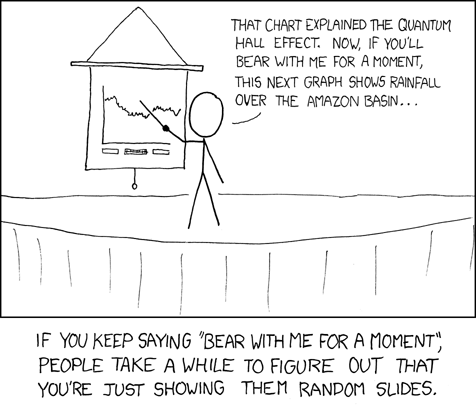
\includegraphics[width=0.9\textheight]{images/xkcd.png}
      \end{center}
    \end{column}
  \end{columns}
\end{frame}
% License Slide
\begin{frame}{Άδεια Χρήσης}
  \begin{center}
    \ccbysa
  \end{center}
  \begin{center}
    Άδεια \href{https://creativecommons.org/licenses/by/4.0/}{Creative Commons Αναφορά Δημιουργού 4.0 Διεθνές (CC BY 4.0)}.  Το παρόν διατίθεται υπό την
    \ccbysa
  \end{center}
  \begin{exampleblock}{Επιτρέπεται στον αποδέκτη:}
    \begin{itemize}
      \item Να μοιραστεί το έργο με άλλους.
      \item Να τροποποιήσει το έργο για προσωπική ή εμπορική χρήση.
      \item Να χρησιμοποιήσει το έργο σε παρουσιάσεις ή δημοσιεύσεις.
      \item Να αναφέρει τον δημιουργό του έργου όταν το χρησιμοποιεί.
    \end{itemize}
  \end{exampleblock}
\end{frame}
\end{document}